\dev {Daphné Kany}{}

\textit{Ce développement vise à prouver certaines propriétés vérifiés par l'algorithme A* selon la nature de l'heuristique utilisée.}

\begin{com}
	On peut se contenter d'écrire l'algorithme dans le plan de la leçon pour gagner du temps
\end{com}

\begin{algorithm}[H]
	\Entree{W la matrice de poids du graphe;
		h le tableau pour l'heuristique;
		$s_{0}$ et $s_{f}$ les sommets initiaux et finaux}
	\Sortie{la distance d'un plus court chemin de $s_{0}$ à $s_{f}$}
	
	$D \gets$ tableau initialisé à $\infty$\\
	$D[s_{0}] \gets$ 0\\
	$P \gets$ file de priorité vide\\
	Ajouter $(s_{0}, h[s_{0}])$ à $P$\\
	\While{$P$ non vide}{
		$(s, \_) \gets$ extract($P$)\\
		\Si{$s = s_{f}$}{retourner $D[s]$}
		\Pour{$s'$ succeseur de $s$}{
			$c \gets D[s] + W[s, s']$\\
			\Si{$c < D[s']$}{
				$D[s'] \gets c$\\
				Ajouter  $(s', c+h[s'])$ à $P$\\
			}
		}
	}
	retourner $Not Found$
	\caption{Algorithme A*}
\end{algorithm}

\paragraph{Notation} Notons $pcc : S^2 \to \N \cup \{-+\infty\}$ la fonction renvoyant la distance d'un plus corut chemin.

\begin{example}
	On applique l'algorithme sur le graphe ci dessous. L'heuristique est précisée pour chaque nœud. 
	\begin{center}
		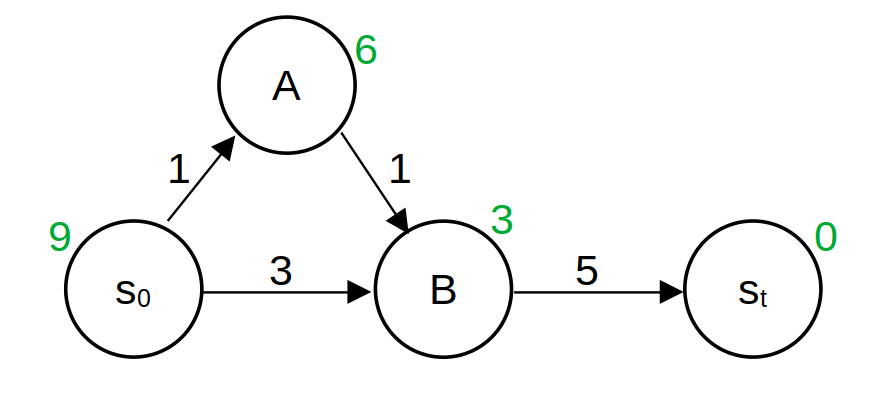
\includegraphics[scale=0.25]{Developpements/Algorithme A etoile/exemple.png}
	\end{center}
	$$D : \:
	\begin{array}{|c|c|c|c|}
		\hline
		\text{$s_{0}$} & \text{A} & \text{B} & \text{$s_{f}$} \\ \hline
		0 & +\infty & +\infty & +\infty \\ \hline
		0 & 1 & 3 & +\infty \\ \hline
		0 & 1 & 3 & 8 \\ \hline
		0 & 1 & 2 & 8 \\ \hline
		0 & 1 & 2 & 7 \\ \hline
	\end{array}
	\quad
	\begin{array}{|c|}
		\hline
		\text{P} \\ \hline
		\text{$s_{0}$ : 9} \\ \hline
		\text{A : 7 ; B : 6} \\ \hline
		\text{A : 7 ; $s_{f}$ : 8} \\ \hline
		\text{B : 7 ; $s_{f}$ : 8} \\ \hline
		\text{$s_{f}$ : 7} \\ \hline
	\end{array}
	$$

\end{example}

\begin{rem}
	Contrairement à l'algorithme de Dijkstra, on peut visiter un même sommet plusieurs fois. 
\end{rem}

\begin{temps}
	3:20 sans écrire l'algo
\end{temps}

\begin{com}
	On peut ensuite modifier l'heuristique du noeud A (par exemple en 8). La nouvelle heuristique n'est pas admissible, et l'algorithme va extraire $s_{f}$ à la quatrième itération, et donc renvoyer une distance qui n'est pas min. 
\end{com}

\begin{theorem}
	Correction de A* : Si l'heuristique est admissible, A* renvoie la distance d'un plus court chemin entre $s_{0}$ et $s_{f}$ s'il existe, et Not found sinon.
\end{theorem}

%\begin{proof}
%	On utilisera l'invariant de boucle suivant : 
%	\begin{center}
%		$\forall{u \in V}, D[u] < +\infty$ ssi u a été inséré dans P. D[u] représente alors la valeur d'un chemin de $s_{0}$ à u.
%	\end{center}
%	
%	\begin{itemize}[label=$\bullet$]
%		\item Supposons qu'il existe un chemin $s_{0} \rightarrow s_{1} \rightarrow ... \rightarrow s_{n} \rightarrow s_{f}$. Montrons que l'algorithme ne renvoie pas $Not Found$, ie $s_{f}$ est inséré dans $P$. \\
%	
%		Raisonnons par l'absurde et supposons $s_{f}$ n'est jamais inséré dans $P$. Soit $s_{i}$ le premier nœud du chemin à ne pas être inséré dans $P$. Alors $s_{i-1}$ a été inséré. Au moment de son extraction, si $s_{i}$ n'est pas dans la file, $D[s_{i}] > D[s_{i-1}] + w(s_{i-1}, s_{i})$ donc il y est inséré, ce qui contredit notre hypothèse. \\
%		Ainsi, s'il existe un chemin de $s_{0}$ à $s_{f}$, l'algorithme ne renvoie pas Not found. \\
%		
%		\item Soit $d$ la valeur renvoyé par A*, et supposons par l'absurde l'existence d'un chemin  $s_{0} \rightarrow s_{1} \rightarrow ... \rightarrow s_{n} \rightarrow s_{f}$ de longueur $d' < d$. \\
%		Montrons par récurrence $\forall{i \in \{1,...,n\}} H_{i} : $ \\
%		«Le sommet $s_{i}$ a été extrait de $P$ avant $s_{f}$ et $D[s_{i}] \le \sum_{k=0}^{i-1}{w(s_{k}, s_{k+1})}$»
%		\begin{itemize}[label=$\star$]
%			\item $H_{1}$:
%			Lors de l'extraction de $s_{0}$, $s_{1}$ est inséré dans $P$ avec la valeur \\
%			$$w(s_{0}, s_{1}) + h(s_{1}) \le w(s_{0}, s_{1}) + dist(s_{1}, s_{f}) \le d' < d $$  \\
%			$s_{1}$ sera donc extrait de $P$ avant $s_{f}$. De plus, $D[s_{1}]$ est mis à jour et vaut désormais $w(s_{0}, s_{1})$.
%			
%			\item Hérédité : Supposons $H_{i}$ et montrons $H_{i+1}$. \\
%			Lors de l'extraction de $s_{i}$, deux cas sont possibles : \\
%			- $D[s_{i+1}] < D[s_{i}] + w(s_{i}, s_{i+1})$ \\
%			Alors $s_{i+1}$ a déjà été inséré dans $P$ avec la valeur 
%			$$ D[s_{i+1}] + h(s_{i+1}) < D[s_{i}] + w(s_{i}, s_{i+1}) + dist(s_{i+1}, s_{f}) \le \sum_{k=0}^{i}{w(s_{k}, s_{k+1})} + dist(s_{i+1}, s_{f}) \le d' < d$$ \\
%			donc $s_{i+1}$ sera extrait de $P$ avant $s_{f}$ et $D[s_{i+1}] \le  \sum_{k=0}^{i}{w(s_{k}, s_{k+1})}$ \\
%			- Sinon, $s_{i+1}$ est mis à jour et vérifie $H_{i+1}$ \\
%		\end{itemize}
%	\end{itemize}
%	En particulier, lors de l'extraction de $s_{n}$, $D[s_{f}] > d'$ et $D[s_{n}] + w(s_{n}, s_{f}) \le d'$. $D[s_{f}]$ est donc mis à jour et vaut désormais $D[s_{n}] + w(s_{n}, s_{f}) \le d'$, ce qui contredit A* renvoie $d$. 
%\end{proof}

\begin{proof}
	Squelette de la preuve : \begin{itemize}[label = $\star$]
		\item On a le variant de boucle suivant : si $D[u] < +\infty$, alors $D[u]$ est la distance d'un chemin de $s_0$ à $u$.
		\item Si il y a un chemin de $s_0$ à $s_f$, alors A* ne renvoie pas NotFound. En effet, par réccurence, chaque élément du chemin est inséré.
		\item A* renvoie $pcc(s_0, s_f)$. \\
		Par l'absurde : On a alors, $D[s_f] > pcc(s_0, s_f)$.\\
		\raisebox{-0.5\height}{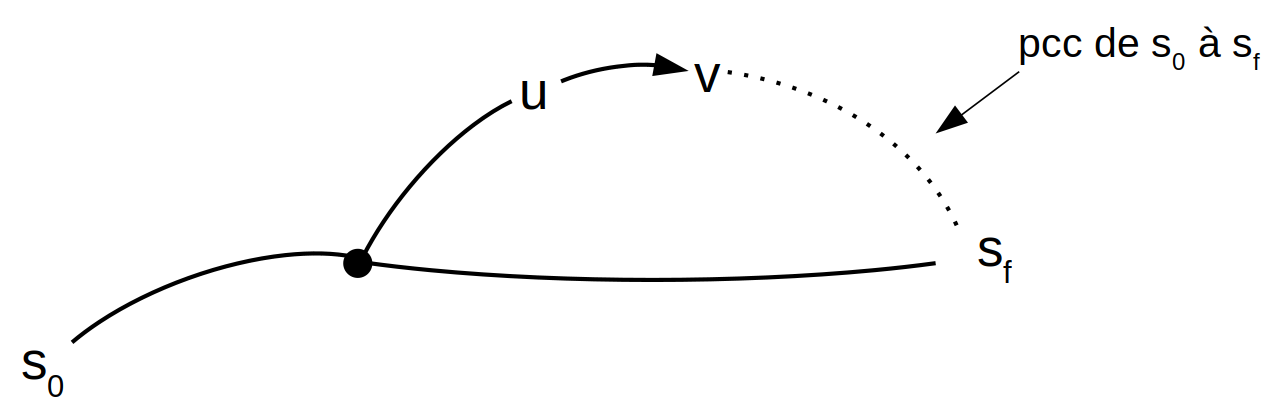
\includegraphics[scale=0.2]{Developpements/Algorithme A etoile/preuve_correction.png}} \begin{tabular}{l}$v$ est le premier sommet du pcc qui n'est \\ pas extrait avec sa valeur minimale. \end{tabular} \\
		Alors dans $P$, $v$ a au plus la valeur $D[u] + w(u,v) + h(v) \leq pcc(s_0, u) + w(u,v) + pcc(v, s_f) = pcc(s_0, s_f) < D[s_f]$ donc $v$ est extrait avec sa valeur minimale avant $s_f$.
	\end{itemize}
\end{proof}
\begin{com}
	Si le temps fait défaut, on peut faire uniquement l'initialisation de la récurrence.
\end{com}

\begin{theorem}
	Si l'heuristique est monotone et vérifie h($s_{f}$) = 0, l'algorithme A* est correct. De plus, chaque sommet u est extrait au plus une fois de $P$ (en ayant à ce stade $D[u] = dist(s_{0}, u)$).
\end{theorem}

\begin{proof}
	\begin{itemize}[label=$\bullet$]
		\item Correction : Soit h une heuristique monotone tq h($s_{f}$) = 0. Montrons que h est admissible. 
		
		Soit $u \rightarrow u_{1} \rightarrow ... \rightarrow u_{n} \rightarrow s_{f}$ un plus court chemin de u à $s_{f}$. \\
		
		$$h(u) \le w(u, u_{1}) + h(u_{1}) \le ... \le h(t) + \sum_{i = 0}^{n-1}{w(u_{i}, u_{i-1})} + w(u_{n}, s_{f}) = dist(u, s_{f})$$
		
		\item On raisonne par l'absurde et on considère v le premier sommet extrait pour lequel $D[v] > dist(s_{0}, v)$. \\
		
		Soit  $s_{0} \rightarrow s_{1} \rightarrow ... \rightarrow s_{n} \rightarrow v$ un plus court chemin de $s_{0}$ à v.
		
		On considère $s_{i}$ le dernier sommet de ce chemin extrait. Alors $s_{i+1}$ non extrait mais inséré dans $P$.  \\
		
		Lors de l'extraction de v, on a : 
		$$ D[v] + h(v) \le D[s_{i+1}] + h(s_{i+1}) \le D[s_{i}] + w(s_{i}, s_{i+1}) + h(s_{i+1}) $$ 
		
		Or $D[s_{i}] + w(s_{i}, s_{i+1}) = dist(s_{0}, s_{i}) + w(s_{i}, s_{i+1}) = dist(s_{0}, s_{i+1})$ \\		
		et $h(s_{i+1}) \le w(s_{i+1}, s_{i+2}) + h(s_{i+2}) \le dist(s_{i+1}, v) + h(v)$ (h monotone)\\
		
		Finalement, on a $ D[v] + h(v) \le dist(s_{0}, s_{i+1}) + dist(s_{i+1}, v) + h(v)$ \\
		donc $ D[v] \le dist(s_{0}, v) $, ce qui est absurde, d'où la conclusion.
	\end{itemize}
\end{proof}

\begin{rem}
On en déduit la complexité de A* dans le cas d'une heuristique monotone : $O((|V|+|E|)log(|V|))$ si la file de priorité est implémentée à l'aide d'un tas-min. 
\end{rem}

